\begin{figure}[h]
  \centering
  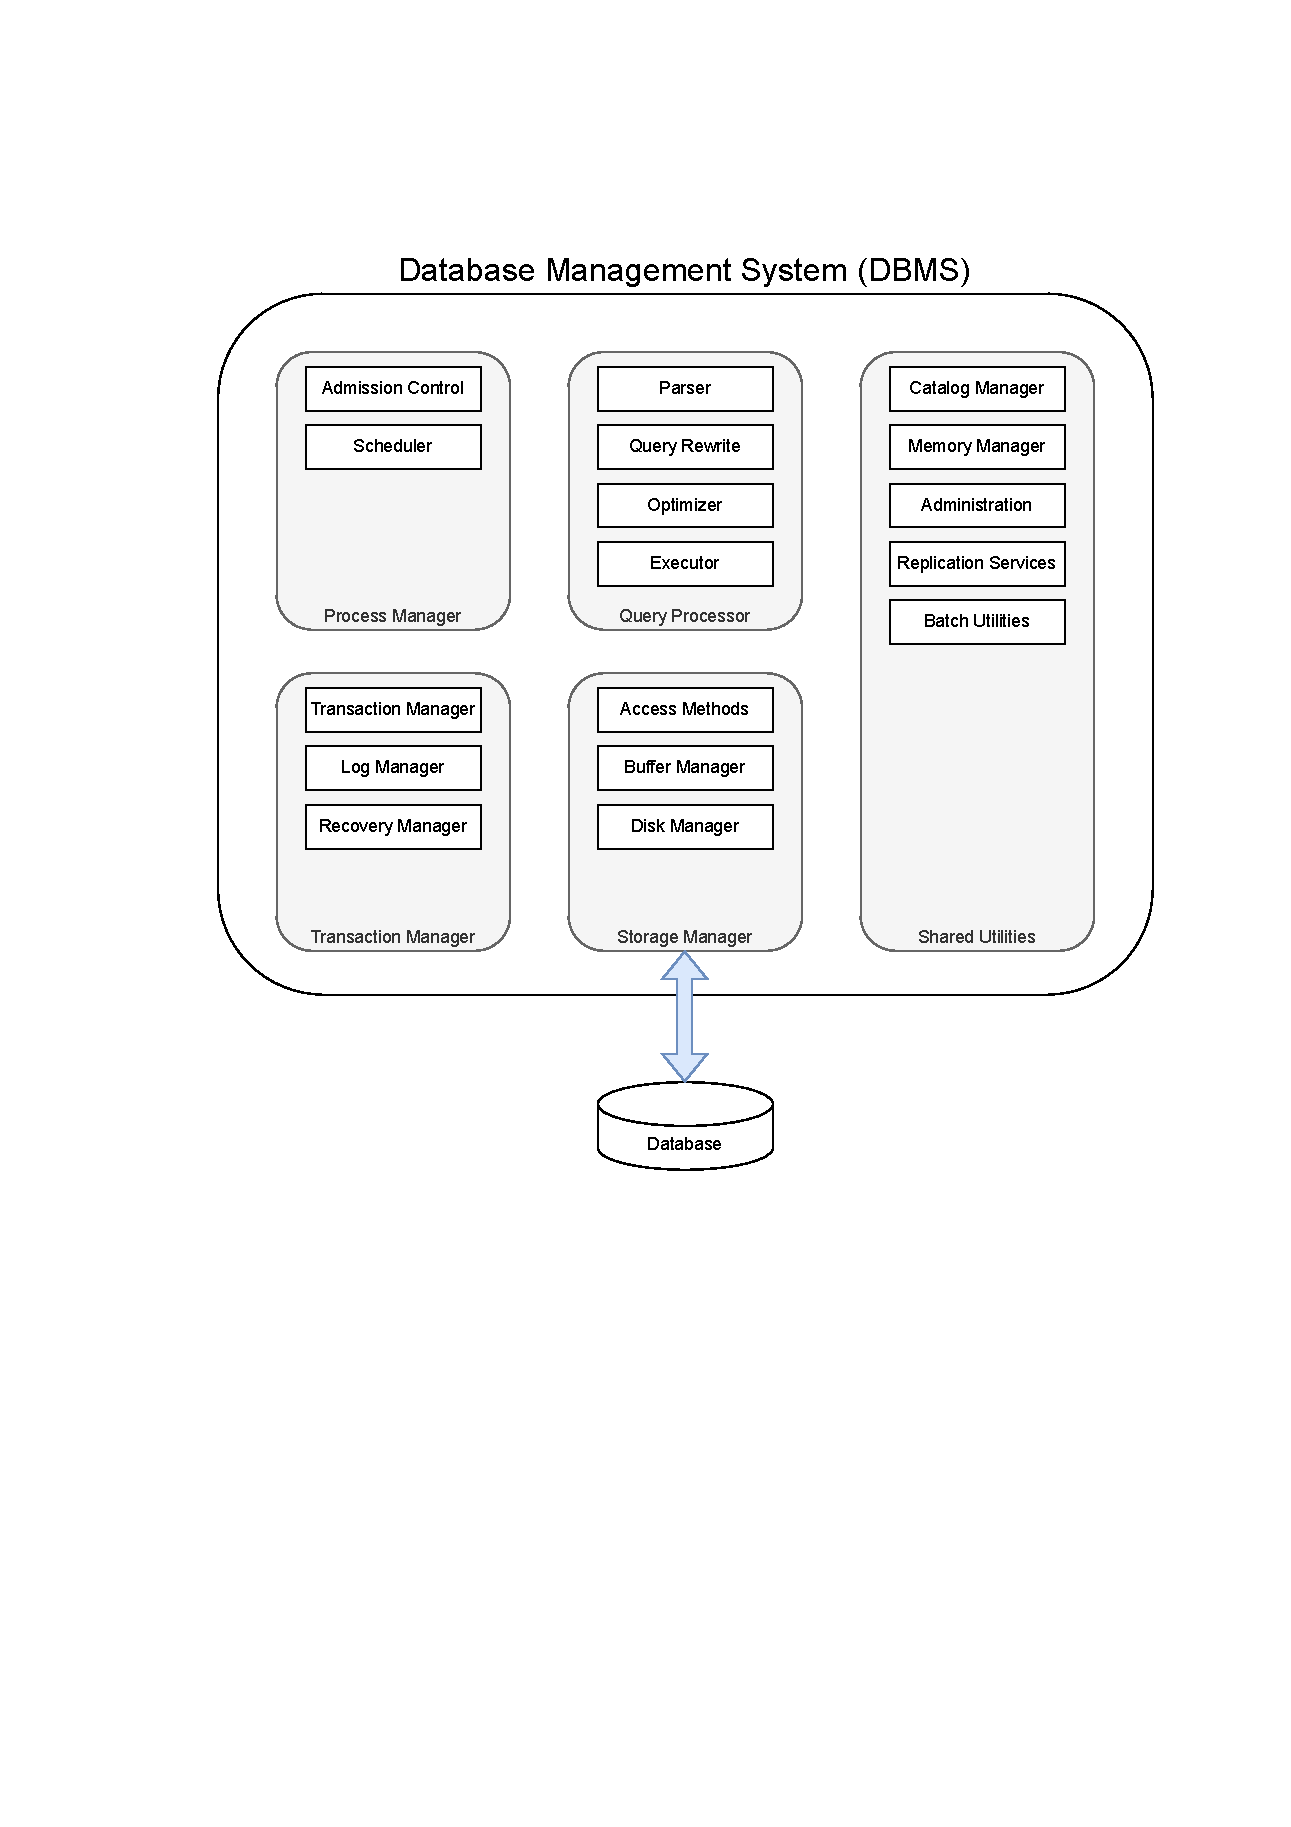
\includegraphics[width=\textwidth, trim=0 310 0 100, clip]{graphs/arq_dbms.pdf}
  \caption{Arquitectura de un DBMS convencional}
\end{figure}

\section{Query Processor}
Para procesar una consulta, es necesario realizar una serie de pasos.
\begin{enumerate}
  \item Parser:
  \begin{itemize}
    \item Valida la consulta (correctitud, autorización, etc).
    \item Convierte la consulta en un formato interno (algebra relacional).
    \item Optimizaciones menores.
  \end{itemize}
  \item Reescritura de la consulta (Query Rewrite):
  \begin{itemize}
    \item "Desanidación" de la consulta (flattening).
    \item Reescritura de la consulta aplicando reglas de algebra relacional.
    \item Creación de un set de planes lógicos optimizados
  \end{itemize}
  \item Optimizador:
  \begin{itemize}
    \item Encuentra el plan físico más eficiente para ejecutar la consulta.
    \item Se consideran varios factores, como el tamaño de cada relación, la distribución de sus datos, distintos métodos de acceso a las relaciones, distintos planes lógicos posibles para la misma consulta, etc.
  \end{itemize}
  \item Ejecutor:
  \begin{itemize}
    \item Ejecutar el plan óptimo generado por el optimizador (pipelining).
  \end{itemize}
\end{enumerate}

\subsection{Plan físico}
El plan físico es similar al plan lógico del álgebra relacional, pero este decide que algoritmo usar para cada operador, planifica la secuencia y el orden a ejecutar de los operadores, además de la forma de acceder a los datos (access path).

\begin{figure}[h]
  \centering
  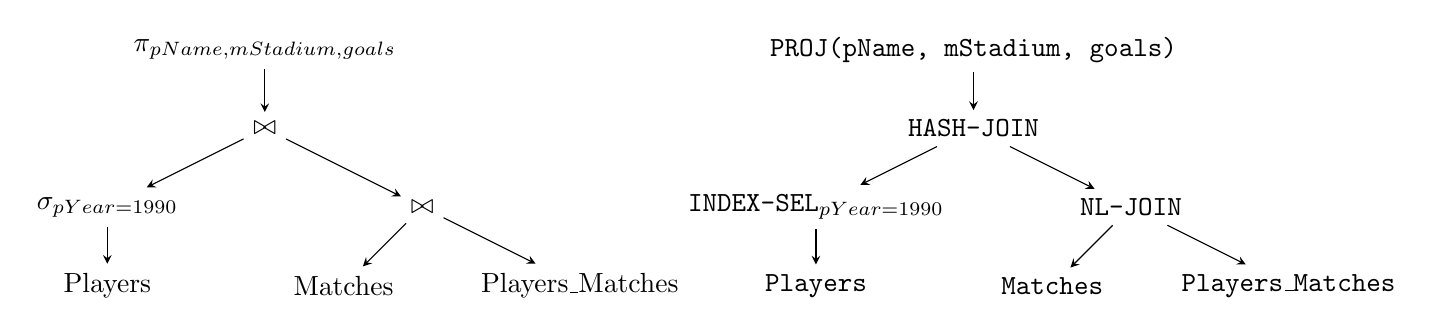
\begin{tikzpicture}
    % Plan lógico
    \node (projection) at (0,0) {$\pi_{\text{pName, mStadium, goals}}$};
    \node (bowtie1) at (0,-1) {$\bowtie$};
    \node (select) at (-2,-2) {$\sigma_{\text{pYear = 1990}}$};
    \node (players) at (-2,-3) {Players};
    \node (bowtie2) at (2,-2) {$\bowtie$};
    \node (matches) at (1,-3) {Matches};
    \node (playersmatches) at (4,-3) {Players\_Matches};
    
    
    \draw[-stealth] (projection) -- (bowtie1);
    \draw[-stealth] (bowtie1) -- (select);
    \draw[-stealth] (select) -- (players);
    \draw[-stealth] (bowtie1) -- (bowtie2);
    \draw[-stealth] (bowtie2) -- (matches);
    \draw[-stealth] (bowtie2) -- (playersmatches);

    % Plan físico
    \node (projectionf) at (9,0) {\texttt{PROJ(pName, mStadium, goals)}};
    \node (bowtie1f) at (9,-1) {\texttt{HASH-JOIN}};
    \node (selectf) at (7,-2) {$\texttt{INDEX-SEL}_{\text{pYear = 1990}}$};
    \node (playersf) at (7,-3) {\texttt{Players}};
    \node (bowtie2f) at (11,-2) {\texttt{NL-JOIN}};
    \node (matchesf) at (10,-3) {\texttt{Matches}};
    \node (playersmatchesf) at (13,-3) {\texttt{Players\_Matches}};
    
    
    \draw[-stealth] (projectionf) -- (bowtie1f);
    \draw[-stealth] (bowtie1f) -- (selectf);
    \draw[-stealth] (selectf) -- (playersf);
    \draw[-stealth] (bowtie1f) -- (bowtie2f);
    \draw[-stealth] (bowtie2f) -- (matchesf);
    \draw[-stealth] (bowtie2f) -- (playersmatchesf);
  \end{tikzpicture}
  \caption{Plan lógico a plan físico}
\end{figure}
\pagebreak

\subsection{Ejecución}
Se empieza a ejecutar en serie el plan físico. Aquí, cada operador retorna tuplas a su padre en el árbol, todo ASAP.

\begin{figure}[h]
  \centering
  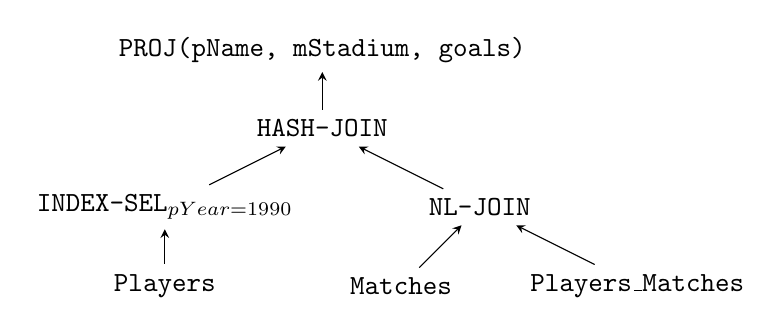
\begin{tikzpicture}
    % Plan físico
    \node (projectionf) at (9,0) {\texttt{PROJ(pName, mStadium, goals)}};
    \node (bowtie1f) at (9,-1) {\texttt{HASH-JOIN}};
    \node (selectf) at (7,-2) {$\texttt{INDEX-SEL}_{\text{pYear = 1990}}$};
    \node (playersf) at (7,-3) {\texttt{Players}};
    \node (bowtie2f) at (11,-2) {\texttt{NL-JOIN}};
    \node (matchesf) at (10,-3) {\texttt{Matches}};
    \node (playersmatchesf) at (13,-3) {\texttt{Players\_Matches}};
    
    
    \draw[stealth-] (projectionf) -- (bowtie1f);
    \draw[stealth-] (bowtie1f) -- (selectf);
    \draw[stealth-] (selectf) -- (playersf);
    \draw[stealth-] (bowtie1f) -- (bowtie2f);
    \draw[stealth-] (bowtie2f) -- (matchesf);
    \draw[stealth-] (bowtie2f) -- (playersmatchesf);
  \end{tikzpicture}
  \caption{Pipelining}
\end{figure}

\section{Storage Manager}
\subsection{Disk Manager}
Esto se encarga del acceso al almacenamiento secundario (Disco duro), y de organizar las tuplas dentro del disco, por medio de heapfiles.

\subsection{Buffer Manager}
Esto se encarga del manejo de los datos en memoria. También se encarga de optimizar la cantidad de accesos que ocurren en el disco duro, ya que el acceso al disco duro es más lento que la RAM. Idealmente se deseará hacer todo en RAM y pasar al almacenamiento persistente al final. Este componente también es importante para todo lo relacionado con transacciones y ACID.

\subsection{Access Methods}
Esto maneja todos los indices y se encarga de mantener una organización eficiente de los datos, tanto en términos de almacenamiento como ordenado para hacer que su acceso sea más rápido.

\section{Transaction Manager}
Este macrocomponente trata de mantener las propiedades ACID (Atomicity, Consistency, Isolation, Durability) en los datos. Particularmente, el Transaction Manager asegura Isolation y Consistency, mientras que el Log Manager y el Recovery Manager aseguran Atomicity y Durability.

\section{Process Manager}
\subsection{Admission Control}
Este componente se encarga de manejar usuarios, permisos, autentificación y otras cosas relacionadas. También es el encargado de asegurar la cantidad de recursos necesarios para que el sistema funcione correctamente.

\subsection{Scheduler}
Este componente se encarga del manejo de procesos y threads dentro de la base de datos, además de paralelizar las consultas.

\section{Shared Utilities}
\begin{itemize}
  \item Catalog Manager: Mantiene la estructura y metadata de los datos. Le permite a la base de datos saber que datos se están almacenando en las distintas relaciones para saber como trabajar con ellos.
  \item Memory Manager: Asigna memoria para distintos componentes de la base de datos.
\end{itemize}

